\begin{enumerate}[label=\thechapter.\arabic*,ref=\thechapter.\theenumi]
    \item The discrete-time Fourier transform of a signal x\sbrak{n} is $X\brak{\Omega}=\brak{1+\cos{\Omega}}e^{-j\Omega}$. Consider that $x_{p}\sbrak{n}$ is a periodic signal of period $N=5$ such that
        \begin{align}
            x_p\sbrak{n}&=x[n],\text{for n= 0, 1, 2}\\
            &=0,\text{for n= 3, 4}
        \end{align}
        Note that $x_p\sbrak{n}=\sum_{k=0}^{N-1}a_{k}e^{j\frac{2\pi}{N}kn}$. The magnitude of the Fourier series coefficient $a_3$ is \rule{3cm}{0.15mm} \brak{\text{Round off to 3 decimal places}}.\hfill(GATE EE 2023)
        \solution
        \newpage

\item Let a frequency modulated (FM) signal : $ x(t) = A \cos(\omega_c t + k_f \int_{-\infty}^{t} m(\lambda) d\lambda)$ , where $ m(t) $is a message signal of bandwidth $ W $. It is passed through a non-linear system with output $y(t) = 2x(t) + 5(x(t))^2 $.
Let $B_T $denote the FM bandwidth. The minimum value of $ \omega_c $ required to recover $ x(t) $ from $ y(t) $ is:\\
\begin{enumerate}[label = (\Alph*)]
\item $B_T + W$ \\
\item $\dfrac{3}{2} B_T$ \\
\item $2B_T + W$ \\
\item $\dfrac{5}{2} B_T$ \\
\end{enumerate}

\solution
\newpage

\item Let an input $x[n]$ having discrete-time Fourier transform
$X(e^{j\Omega}) = 1 - e^{-j\Omega} + 2e^{-3j\Omega}$
be passed through an LTI system. The frequency response of the LTI system is 
$H(e^{j\Omega}) = 1 - \frac{1}{2} e^{-2j\Omega}$
The output $y[n]$ of the system is \\ \hfill(GATE EC 2023)
\solution 
\newpage
\item The Fourier transform $X(\omega)$ of $x(t) = e^{-t^2}$ is\\
Note:$\int_{-\infty}^{\infty} e^{-y^2} \,dy = \sqrt{\pi}$ \\  
A) $\sqrt{\pi} e^{\frac{\omega^2}{2}}$ \\
B) $\frac{e^{\frac{-\omega^2}{4}}}{2\sqrt{\pi}}$ \\
C) $\sqrt{\pi} e^{\frac{-\omega^2}{4}}$ \\
D) $\sqrt{\pi} e^{\frac{-\omega^2}{2}}$\\
\hfill Gate 2023 EC Question 28
\newpage

 \item Let $x(t) = 10 \cos(10.5 \omega t)$ be passed through an LTI system with impulse response $h(t) = \pi\left(\frac{\sin(\omega t)}{\pi t}\right)^2 \cos(10 \omega t)$ . The output of the system is:\\ \hfill(GATE EC 2023)
 \solution
 \newpage
 
 \item Q27) Let m\brak{\text{t}} be a strictly band-limited signal with bandwidth B and energy E. Assuming $\omega_0$ = 10B, the energy in the signal $\text{m}\brak{t}\text{cos}\brak{\omega_0\text{t}}$\\[1ex]

	\brak{A}\ $\frac{E}{4}$\\[1ex]

		\brak{B}\ $\frac{E}{2}$\\[1ex]

		\brak{C}\ $E$\\[1ex]

		\brak{D}\ $2E$ \qquad\qquad\qquad\quad\qquad\qquad\qquad\qquad\brak{\text{GATE EC 2023}}\\

\solution

\newpage

\item The following function is defined over the integral $[-L,L]:$
    $$f\brak{x}=px^4+qx^5$$
It is expressed as a Fourier series,
    $$f\brak{x}=a_0+\sum_{n=1}^{\infty}\cbrak{a_n\sin\brak{\frac{\pi x}{L}}+b_n\cos\brak{\frac{\pi x}{L}}}$$

which options amongst the following are true?
\begin{enumerate}[label=(\alph*)]
    \item $a_n$, $n=1,2,..,\infty$ depend on $p$
    \item $a_n$, $n=1,2,..,\infty$ depend on $q$
    \item $b_n$, $n=1,2,..,\infty$ depend on $p$
    \item $b_n$, $n=1,2,..,\infty$ depend on $q$
\end{enumerate}
\hfill(GATE 2023 CE Question 25)\\
\solution
\newpage
\item A continuous real-valued signal $x\brak{t}$ has finite positive energy and $x\brak{t} = 0$, $\forall$ $t < 0$. From the list given below, select ALL the signals whose
continuous-time Fourier transform is purely imaginary.\\
\begin{enumerate}
\item$x\brak{t} + x\brak{-t}$
\item$x\brak{t} - x\brak{-t}$
\item$j\brak{x\brak{t} + x\brak{-t}}$
\item$j\brak{x\brak{t} - x\brak{-t}}$
\end{enumerate}
\hfill{(GATE IN 2023)}\\
\solution
\item Let $x_1(t) = u(t + 1.5) - u(t - 1.5)$ and $x_2(t)$ is shown in the figure below. For $y(t) = x_1(t) * x_2(t)$, the $\int_{-\infty}^{\infty} y(t) \, dt$ is \underline{\hspace{2cm}}.\\

\begin{figure}[htbp]
    \centering
    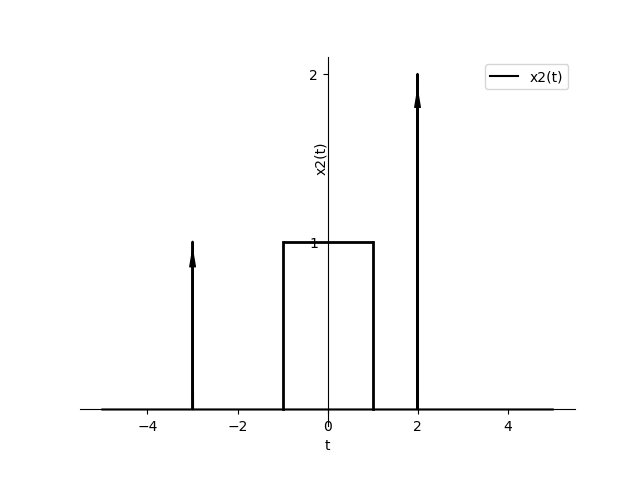
\includegraphics[width=0.5\textwidth]{2023/EC/58/figs/gatefig.png}
    \caption{Figure}
    \label{fig:graph}
\end{figure}

\hfill{(GATE IN 2023)}\\
\solution
\pagebreak
\item Consider a discrete-time signal with period $N=5$. Let the discrete-time Fourier series (DTFS) representation be $ x[n] = \sum\limits_{k=0}^{4} a_k e^{\frac{jk2\pi n}{5}} $where $a_0=1$, $a_1=3j$, $a_2=2j$, $a_3=-2j$, $a_4=-3j$. The value of the sum $\sum\limits_{n=0}^{4}x[n] \sin\left(\frac{4\pi n}{5}\right) $is\\
(A) -10\\
(B) 10\\
(C) -2\\
(D) 2\\
\hfill Gate 2023 EC 47
\solution
\pagebreak
\item A continuous time, band-limited signal $x(t)$ has its Fourier transform described by:
\[ X(f) = \begin{cases} 
1 - \frac{|f|}{200} & \text{if } |f| \leq 200 \\
0 & \text{if } |f| > 200 
\end{cases} \]
The signal is uniformly sampled at a sampling rate of 600 Hz. The Fourier transform of the signal is $X_s(f)$. What is the value of $\frac{X_s(600)}{X_s(500)}$? \\\hfill{(GATE 2023 BM)}
\solution
\pagebreak
 \item The magnitude and phase plots of an LTI systems are shown in figure. Find the transfer function.
\begin{figure}[!h]
    \centering
    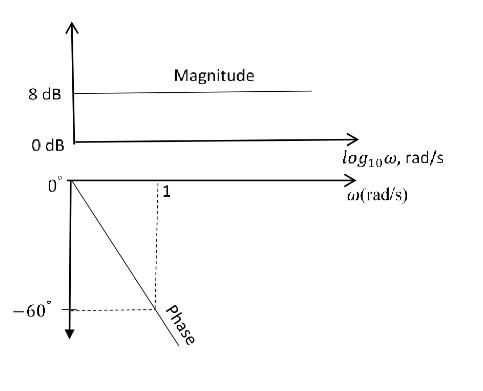
\includegraphics[width=\columnwidth]{2023/EE/36/figs/gate.png}
    \caption{}
    \label{fig:EEgatefig36.23}
\end{figure}
\begin{enumerate}
    \item $2.511 e^{-0.0032s}$\\
    \item $\frac{e^{-2.514s}}{s+1}$\\
    \item $1.04e^{-2.514s}$\\
    \item $2.511 e^{-1.047s}$\\
\end{enumerate} \hfill{(GATE EE 23)}\\

\solution
\pagebreak
\item A system is described by the following differential equation
    \[
    0.01 \frac{d^2y(t)}{dt^2} + 0.2\frac{dy(t)}{dt} + y(t) = 6x(t)
    \]
    where time \( t \) is in seconds. If \( x(t) \) is the unit step input applied at \( t = 0 \) s to this system, the magnitude of the output at \( t = 1 \) s is \(\underline{\hspace{2cm}}\). (Round off the answer to two decimal places.)\hfill {Gate-2023.BM}
    \solution
    \pagebreak
\end{enumerate}
